\chapter{Formato del Proyecto Fin de Grado}
\label{ch:presentacion}


% El siguiente es el texto que aparece en el encabezamiento del proyecto fin de grado (si se quiere que sea distinto al nombre del capítulo))
\chaptermark{PFG}


\section{Formato}
\label{secc:formato}

Aquí deberás de escribir tu documento. Las secciones con la palabra \texttt{section} (\verb+\section{Formato}+) y las subsecciones con la palabra  \texttt{subsection} (\verb+\subsection{Listas}+).

En la web encontrarás documentación extensa sobre \LaTeX{}. Algunas direcciones:  


\vspace{0.25cm}

\url{http://es.wikibooks.org/wiki/Manual\_de\_LaTeX}

\url{http://en.wikibooks.org/wiki/LaTeX}

\url{http://itsas.ehu.es/workgroups/latex/recetas}

\vspace{0.25 cm}

En este documento se describen algunas ideas básicas para dar formato en \LaTeX{}. Se recomienda abrir el documento original \emph{5-examples-es.tex} para ver el código. 

Para escribir notas en el documento origen y que no se vean en el resultado hay que usar el símbolo  ``\%'' por delante de la nota.


% Así


\subsection{Listas}
\label{subsecc:listas}

Se usan dos tipos de listas:

\vspace{0.25 cm}

Numeradas:
\begin{enumerate}
	\item Uno
	\item Dos
	\item Tres
\end{enumerate}

Código:

\vspace{0.25 cm}

\begin{minipage}{8cm}
\begin{verbatim}
  \begin{enumerate} 
  \item Uno
  \item Dos 
  \item Tres
  \end{enumerate} 
\end{verbatim}
\end{minipage}

\vspace{0.5 cm}

Sin numerar:
\begin{itemize}
	\item Puerta
	\item Manzana
	\item Árbol
\end{itemize}

Código:
\vspace{0.5 cm}

\begin{minipage}{8cm}
\begin{verbatim}
  \begin{itemize}
  \item Puerta
  \item Manzana
  \item árbol
  \end{itemize}
\end{verbatim}
\end{minipage}

\subsection{Tablas}
\label{subsecc:tablas}

\LaTeX{} coloca las tablas y las figuras (floats) mediante un algoritmo interno por lo que a veces es difícil que queden donde queramos (se colocan en el sitio más adecuado según el algoritmo). Se pueden dar instrucciones para que coloque estos elementos (ver htbp en el código). 


\begin{table}[ht]
% Opciones h (here), t (top), b (botton), p (next page)
% Preferencias: [htbp] (poner en el orden deseado)
% Obligar a poner el float aquí: [!h] 
\begin{center}
   \begin{tabular}{|l|cl|}
      \hline \bf Asignatura & \bf Cuatrimestre & \bf Créditos \\ \hline
              Programación Básica & 1  & 6 \\
              Análisis Matemático & 1 & 6 \\
              Metodología de la Programación & 2  & \\
              Cálculo & 2 & 6 \\
       \hline
   \end{tabular}
\end{center}
\caption{\label{Asig-1} Algunas asignaturas del grado en II. }
\end{table}

\vspace{4 cm}

Código:

\vspace{0.5 cm}

\begin{minipage}{8cm}
\begin{verbatim}
\begin{table}[ht]
% Opciones h (here), t (top), b (botton), p (next page)
% Preferencias: [htbp] (poner en el orden deseado)
% Obligar a poner el float aquí: [!h] 
\begin{center}
   \begin{tabular}{|l|cl|}
      \hline \bf Asignatura & \bf Cuatrimestre & \bf Créditos \\ 
      \hline
              Programación Básica & 1  & 6 \\
              Análisis Matemático & 1 & 6 \\
              Metodología de la Programación & 2  & \\
              Cálculo & 2 & 6 \\
       \hline
   \end{tabular}
\end{center}
\caption{\label{Asig-1} Algunas asignaturas del grado en II. }
\end{table}
\end{verbatim}
\end{minipage}

\vspace{0.5 cm}

Mediante la etiqueta \verb+\label{}+ que puedes ver en el código puedes hacer referencias a las tablas y figuras sin tener que conocer su orden de aparición. Para ello se usa la instrucción \verb+\ref{Asig-1}+. Por ejemplo, ``En la tabla \ref{Asig-1} se pueden ver algunas asignaturas de primero'' (En la tabla \verb+\ref{Asig-1}+ se pueden ver \ldots).

\vspace{0.5 cm}

\subsection{Figuras}
\label{subsecc:figuras}

A continuación en la figura \ref{fig:infor-hall} se puede ver el hall de la Facultad de Informática:

\begin{figure}[htbp] 
  \begin{center} 
    \scalebox{0.4}{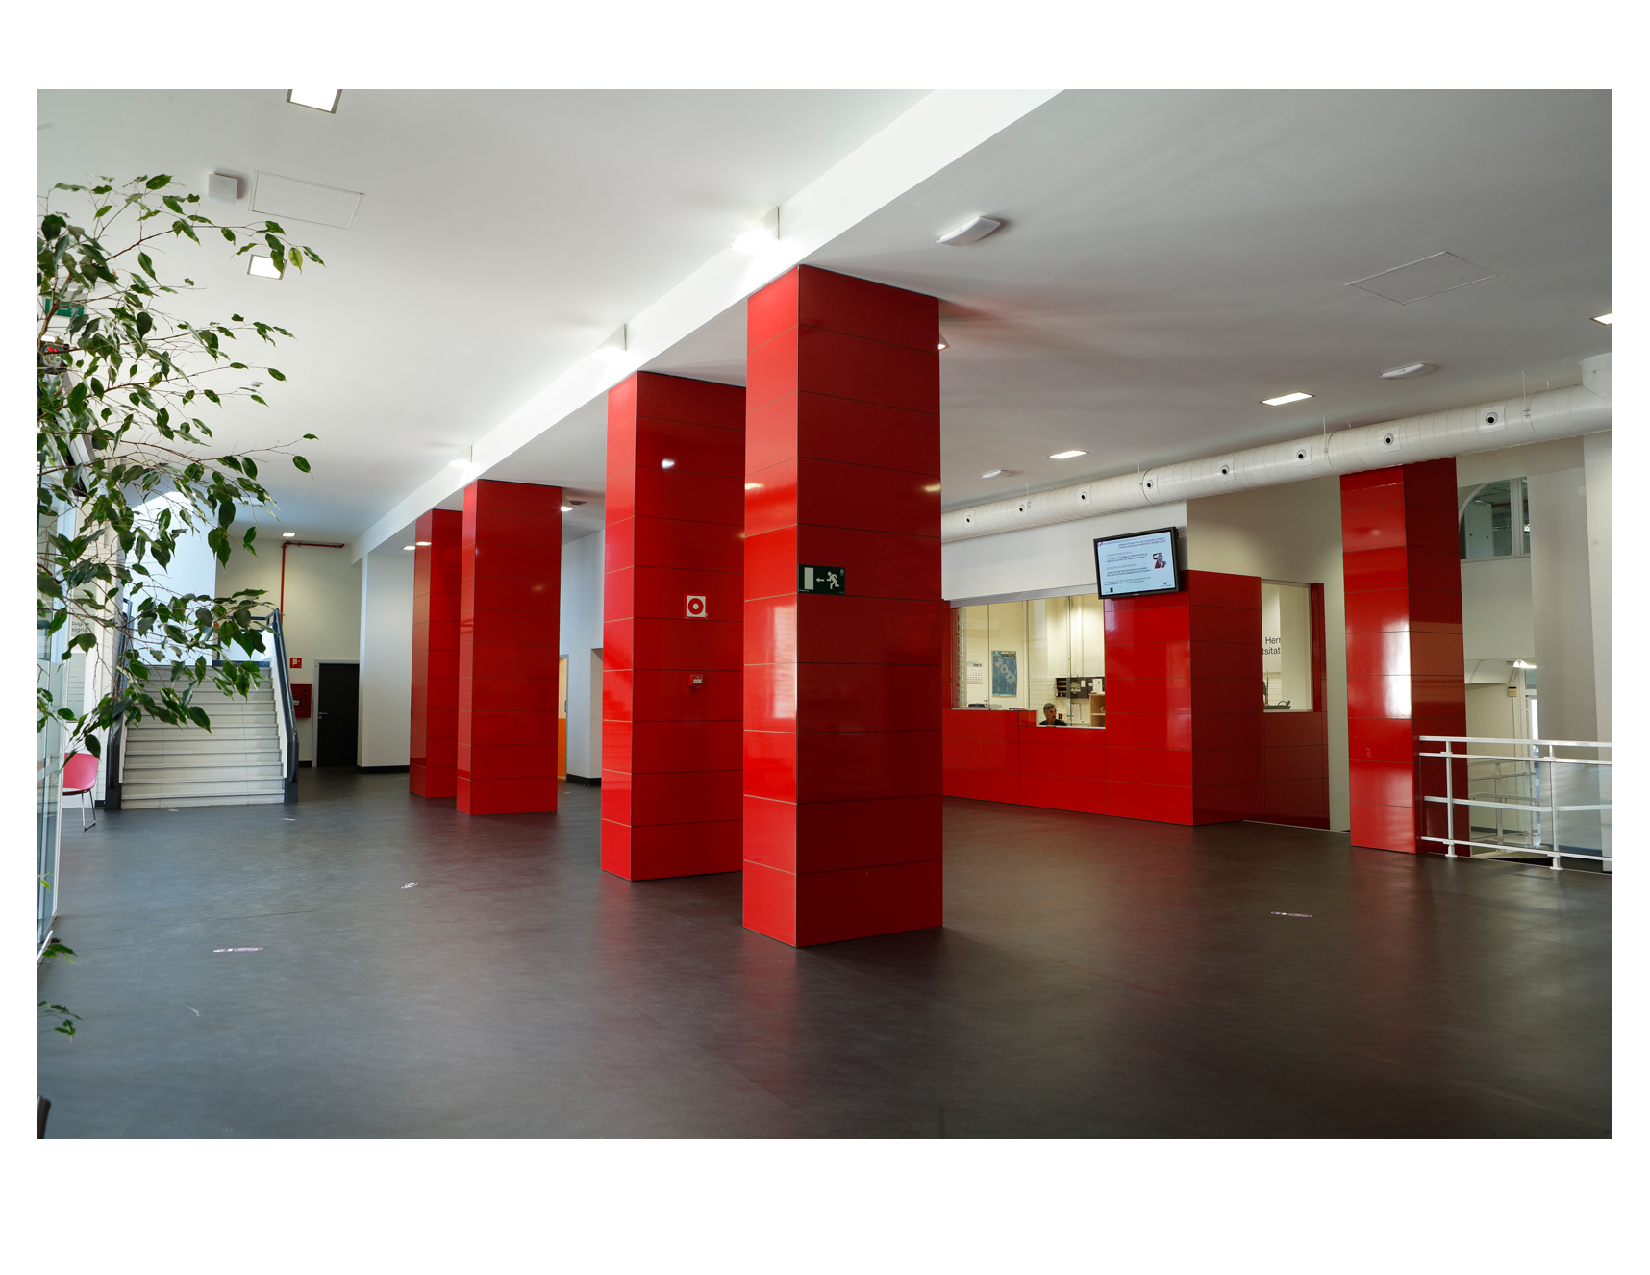
\includegraphics{figs/hall.pdf}} 
    \caption{Hall de la \emph{Facultad de Informática}.} 
    \label{fig:infor-hall} 
  \end{center} 
\end{figure}

Código:

\vspace{0.5 cm}

\begin{minipage}{8cm}
\begin{verbatim}
\begin{figure}[htbp] 
  \begin{center} 
    \scalebox{0.4}{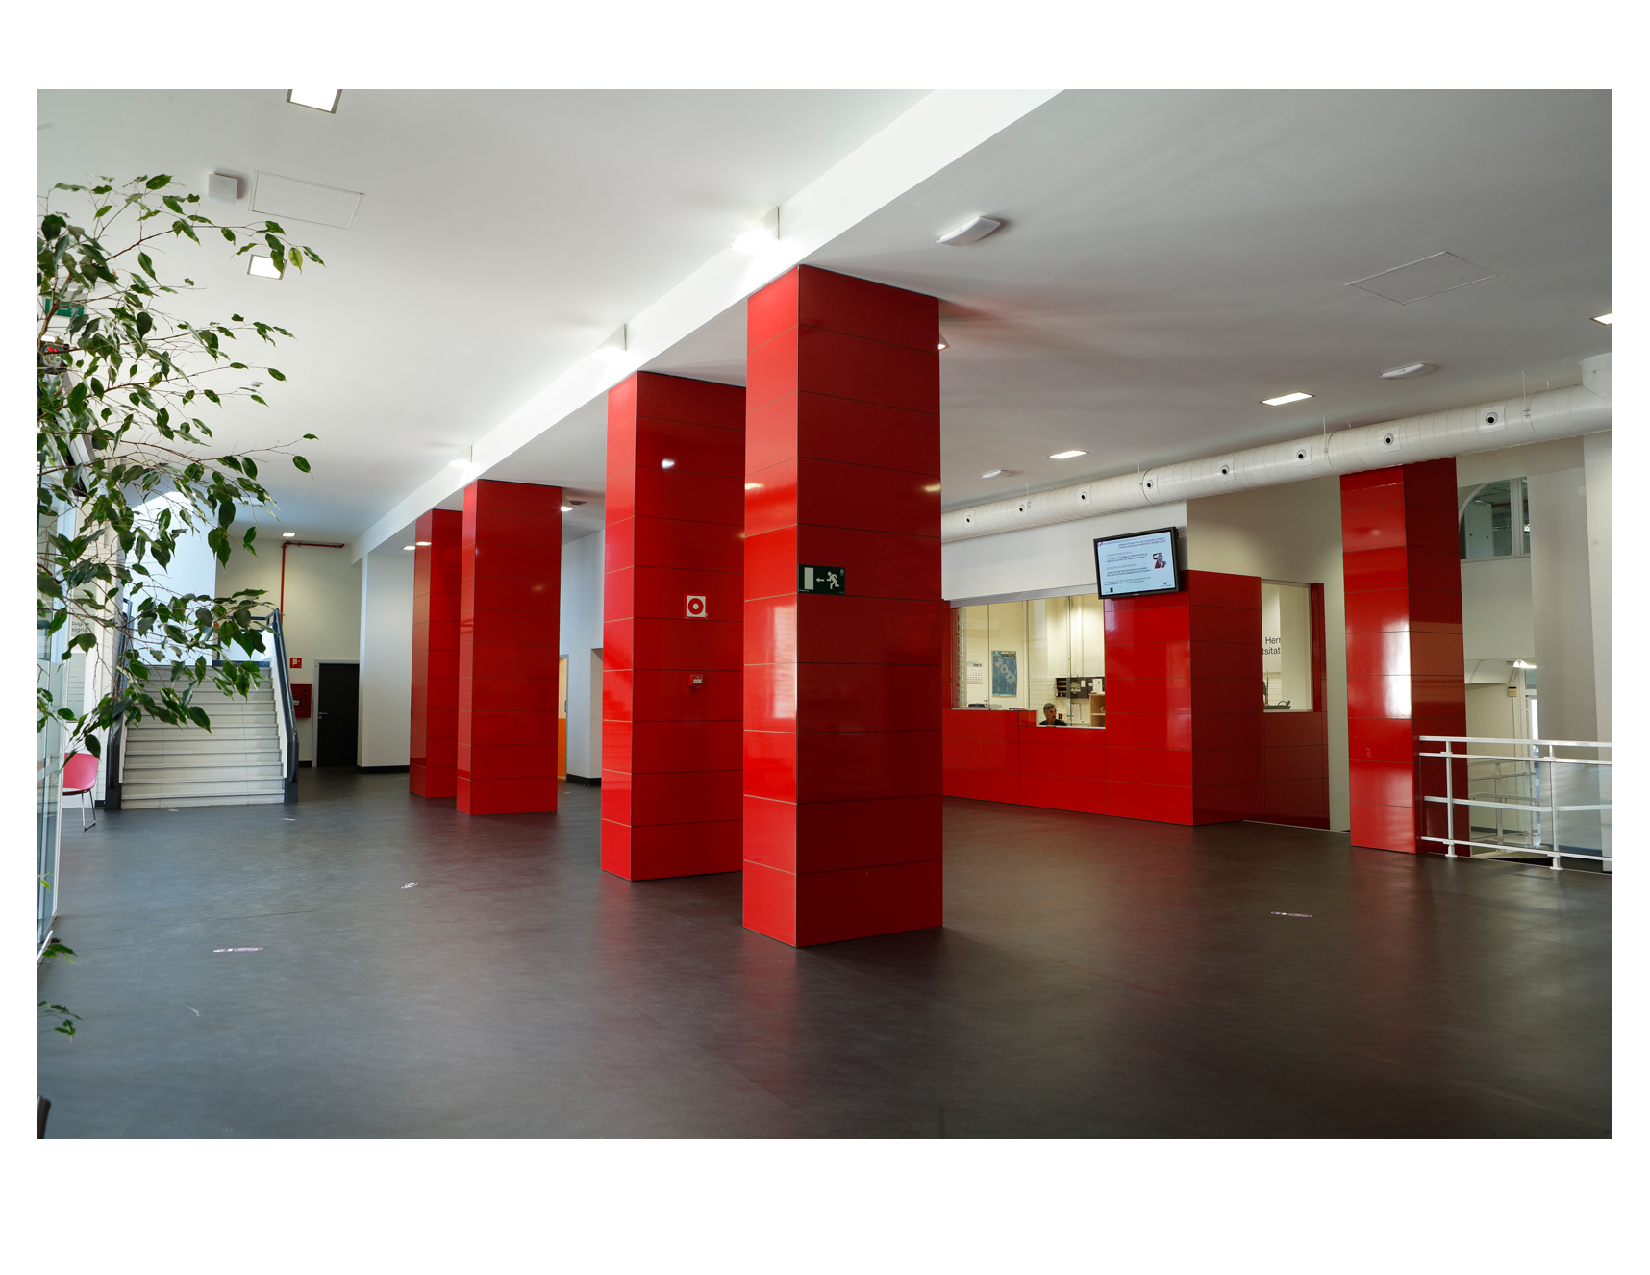
\includegraphics{figs/hall.pdf}} 
    \caption{Hall de la \emph{Facultad de Informática}.} 
    \label{fig:infor-hall} 
  \end{center} 
\end{figure}
\end{verbatim}
\end{minipage}


\subsection{Tipos de letras}
\label{subsecc:letras}


El texto lo puedes escribir en \textbf{negrita} (\verb+\textbf{negrita}+), en \emph{cursiva} (\verb+\emph{cursiva}+) o en \textit{italica} (\verb+\textit{italica}+). Pero también se pueden escribir si así te parece, en \textsc{letras mayúsculas peque\~{n}as} \\(\verb+\textscs{letras mayúsculas peque\~{n}as}+).


Además puedes cambiar el tama\~{n}o de las letras:

\begin{itemize}
 \item {\tiny de esta manera}(\verb+{\tiny de esta manera}+)
 \item {\scriptsize de esta manera} (\verb+{\scriptsize de esta manera}+)
 \item {\footnotesize de esta manera} (\verb+{\footnotesize de esta manera}+)
 \item {\small de esta manera} (\verb+{\small de esta manera}+)
 \item {\normalsize de esta manera} (\verb+{\normalsize de esta manera}+)
 \item {\large de esta manera} (\verb+{\large de esta manera}+)
 \item {\Large de esta manera} (\verb+{\Large de esta manera}+)
 \item {\LARGE de esta manera} (\verb+{\LARGE de esta manera}+)
 \item {\huge de esta manera} (\verb+{\huge de esta manera}+)
 \item {\Huge de esta manera} (\verb+{\Huge de esta manera}+)
 \item \ldots 
\end{itemize}


\subsection{Bibliografía}
\label{subsecc:biblio}

La bibliografía se maneja de manera muy adecuada en \LaTeX{}. Las referencias a libros, artículos o páginas web se almacenan en un fichero aparte.

En este documento, según lo que se describe en ``main.tex'' las referencias bibliográficas se almacenan en el fichero llamado  \emph{biblio} (\verb+\bibliography{biblio}+) del siguiente modo:
 
\vspace{0.25 cm}

Código:

\vspace{0.25 cm}

\begin{minipage}{8cm}
\begin{verbatim}
@book{DBLP:books/aw/Lamport86,
	author    = {Leslie Lamport},
	title     = {LaTeX: User's Guide {\&} Reference Manual},
	publisher = {Addison-Wesley},
	year      = {1986},
	isbn      = {0-201-15790-X},
	bibsource = {DBLP, http://dblp.uni-trier.de}
}
\end{verbatim}
\end{minipage}

\vspace{0.25 cm}

Para hacer alusión en el texto a esta referencia, por ejemplo \cite{DBLP:books/aw/Lamport86}, debemos escribir lo siguiente: \verb+\cite{DBLP:books/aw/Lamport86}+.

\subsection{Footnotes}
\label{subsecc:notas-al-pie}

Las footnote o notas al pie\footnote{Una peque\~{n}a nota como ejemplo.} se ponen con el comando \verb+\footnote{}+.



% Mediante los siguientes comandos, podrás compilar el conjunto de ficheros desde este mismo documento


%%% Local Variables: 
%%% mode: latex
%%% TeX-master: "../Principal"
%%% End: 


















% line in order to check if utf-8 is properly configured: áéíóúñ
